\begin{frame}[fragile]{Visualização de um grafo}

    \begin{figure}
        \centering

        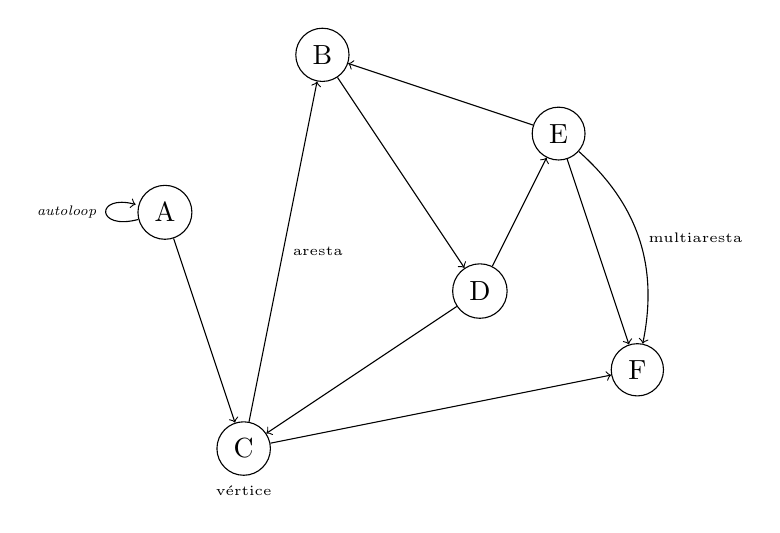
\begin{tikzpicture}
            \coordinate (A) at (0, 3);
            \coordinate (B) at (2, 5);
            \coordinate (C) at (1, 0);
            \coordinate (D) at (4, 2);
            \coordinate (E) at (5, 4);
            \coordinate (F) at (6, 1);

            \node[draw,circle] (A1) at (A) { A };
            \node[draw,circle] (B1) at (B) { B };
            \node[draw,circle] (C1) at (C) { C };
            \node[draw,circle] (D1) at (D) { D };
            \node[draw,circle] (E1) at (5, 4) { E };
            \node[draw,circle] (F1) at (6, 1) { F };

            \path (A1) edge[loop left] node[anchor=east] { \tiny \it autoloop } (A1);
            \draw[->] (A1) -- (C1);
            \draw[->] (C1) -- node[anchor=west] { \tiny aresta } (B1);
            \draw[->] (B1) -- (D1);
            \draw[->] (C1) -- (F1);
            \draw[->] (D1) -- (C1);
            \draw[->] (D1) -- (E1);
            \draw[->] (E1) -- (F1);
            \draw[->] (E1) -- (B1);
            \draw[->] (E1) to [bend left] node[anchor=west] { \tiny multiaresta } (F1);

            \node[anchor=north] at (C1.270) { \tiny vértice };
        \end{tikzpicture}

    \end{figure}

\end{frame}
